%04chapterSelbsteinsch.tex
\chapter{Teamgrundlagen}
\label{sec:Teamgrundlagen}

\section{Organigramm}

\section{Teamvertrag}

Der folgende Teamvertrag wurde am Anfang des Projektes niedergeschrieben. Spätere Änderungen werden in diesem Abschnitt und im Abschnitt \ref{sec:Vorgehen} beschrieben.

\vspace{20mm}
\rule{\textwidth}{1pt}

Das Ziel dieses Dokuments ist das Festlegen allgemeiner Regeln, die für die zukünftige Teamarbeit als verbindlich gelten.\\

\begin{center}

\includegraphics[scale=0.25]{img/clock}\\
\end{center}


\begin{itemize}
\item Pünktlichkeit ist sehr wichtig. Bei mehr als 10 Minuten Verspätung, ist dies den anderen per WhatsApp zu melden
\end{itemize}

\begin{center}

\includegraphics[scale=1.1]{img/work}\\
\end{center}

\begin{itemize}
\item Falls ein Auftrag ohne akzeptable Begründung nicht erledigt wird, muss dieser auf die nächste Woche nachgeholt werden. Falls er auch dann nicht erledigt wurde, wird eine Konsequenz mit dem Dozenten erarbeitet
\end{itemize}

\begin{center}

\includegraphics[scale=0.3]{img/lecture}\\
\end{center}

\begin{itemize}
\item Wenn nicht anders abgemacht, treffen wir uns jeden Montag in der Vorlesung. Falls weitere Termine notwendig sind, werden zusätzliche Sitzungen einberufen \\
\end{itemize}

\begin{center}

\includegraphics[scale=0.25]{img/communication}\\
\end{center}

\begin{itemize}
\item Als Kommunikationskanäle dienen unsere WhatsApp-Gruppe und das schulinterne E-Mail. Als Datenablage und Versionskontrolle verwenden wir GitHub. Bei grösseren Files wird die eingerichtete OneDrive-Cloud hinzugezogen\\\\
\end{itemize}

\begin{center}

\includegraphics[scale=1.2]{img/doc}\\
\end{center}

\begin{itemize}
\item Um Dokumente zu setzen, wird \LaTeX verwendet. Die nötigen Vorlagen werden, falls als sinnvoll erachtet, erstellt
\end{itemize}

\begin{center}
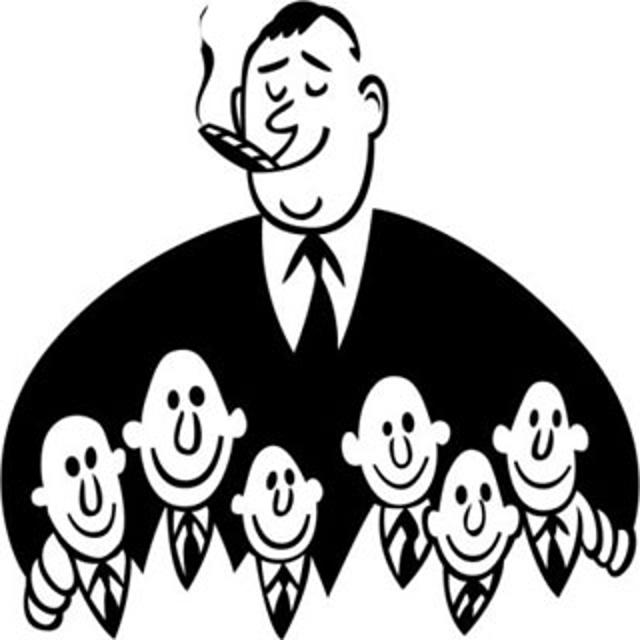
\includegraphics[scale=0.12]{img/boss}\\
\end{center}

\begin{itemize}
\item Da unsere Gruppenstruktur keinen eigentlichen Chef aufweist, werden folgende Verantwortungsbereiche definiert (Änderungen bei Einstimmigkeit vorbehalten):\\


\begin{itemize}
\item Projektkoordinator: Pascal Horat
\item LaTeX-Vorlagen: Pascal Horat
\item MS-Project: Steve Gerome Kamga
\item Git/Github: Gökhan Kaya  
\item Projektbericht: Pascal Horat
\item Kostenveranschlagung: Gökhan Kaya
\item Vortragsplanung: Steve Gerome Kamga
\item Teamreview: alternierend
\item Sitzungschef: alternierend
\end{itemize}
\end{itemize}


\begin{center}

\includegraphics[scale=0.3]{img/voteHand}\\
\end{center}

\begin{itemize}
\item Jede Meinungsverschiedenheit wird besprochen und falls keine Einigung erzielt werden kann, nach relativer Mehrheitswahl entschieden\\\\
\end{itemize}

\begin{center}

\includegraphics[scale=0.3]{img/performance}\\
\end{center}

\begin{itemize}
\item Unsere Teamphilosophie ist es, mit einem gegebenen Zeitaufwand ein möglichst gutes Produkt abzuliefern. Das Ziel dabei ist, möglichst viele Arbeiten während der Vorlesungszeit erledigen zu können\\\\
\end{itemize}

\begin{center}

\includegraphics[scale=0.7]{img/quality}\\
\end{center}

\begin{itemize}
\item Falls eine Person die angestrebte Qualität vernachlässigt, wird eine zweiwöchige Frist angesetzt. Hat sich in dieser Frist die Qualität der Produkte nicht verbessert, werden weitere Schritte in Absprache mit dem Dozenten eingeleitet\\\\
\end{itemize}

%\begin{tabular}{p{6.5cm}p{6.5cm}p{6.5cm}}
\begin{tabular}{p{4cm}p{5cm}p{5.5cm}}
Pascal Horat & Steve Gerome Kamga & Gökhan Kaya\\

\includegraphics[scale=0.6]{img/unterschriftPascal}&

\includegraphics[scale=0.6]{img/unterschriftGerome}&

\includegraphics[scale=0.6]{img/unterschriftGoekhan}
\end{tabular}

\section{Teamrollen}

Im Teamreview 2 wurde eine Selbsteinschätzung gemäss Belbin-Verfahren durchgeführt. Anschliessend kamen jeweils noch Fremdeinschätzungen unsererseits dazu. Der Vorgang, die Resultate und eine ausführliche Analyse mit Vergleichen sind alle im Teamreview 2 zu finden. 

\section{Teameffizienz}

Anfangs wurden alle Arbeiten im Plenum erledigt. Ein Grund dafür könnte sein, dass wir uns nicht ganz sicher waren, was genau wie zu erledigen war. So konnten wir uns ständig austauschen. Das Problem war jedoch, dass sich dieses Vorgehen als sehr ineffizient herausstellte. Der Teamvertrag musste also in einigen Punkten revidiert werden. Insbesondere wurde nun Pascal der Teamchef und verteilte die Aufträge, während wir die Aufträge so selbstständig wie möglich zu erledigen versuchten. Dies führte zu einer deutlichen Effizienzsteigerung. \\
Weiter litt die Teameffizienz deutlich daran, dass Pascal einen Monat im Militärdienst war und Gerome einige Schwierigkeiten mit der Sprache, Github und Latex hatte. \\
Nichtsdestotrotz verlief die Zusammenarbeit ohne zwischenmenschliche Schwierigkeiten, was vor allem für Gökhan ein sehr wichtiger Faktor darstelle.  \\
Eine detaillierte Auseinandersetzung dazu ist im Teamreview 3 zu finden.  
